\section{Experiment Tracking}

% --- SLIDE 1: THE PROBLEM ---
\begin{frame}{The Spreadsheet Everyone Starts With}

    \centering
    \begin{columns}[T]
        \begin{column}{0.5\textwidth}
            \begin{tcolorbox}[colback=red!5, colframe=red!50, title=\small \texttt{results\_final\_v3\_REAL.xlsx}]
                \scriptsize
                \begin{tabular}{lll}
                    \textbf{run} & \textbf{lr} & \textbf{acc} \\
                    \hline
                    exp1        & 0.01  & 0.83 \\
                    exp1b       & 0.01  & 0.86 \\
                    exp2\_new   & 0.001 & 0.91 \\
                    final       & ?     & 0.94 \\
                    final2      & ?     & 0.93 \\
                \end{tabular}
                \vspace{0.5em}
                \\ \textit{Which commit? Which data? Which split? Which preprocessing?}
            \end{tcolorbox}
        \end{column}
        \begin{column}{0.46\textwidth}
            \small
            \textbf{What always goes wrong}
            \begin{itemize}
                \item The best number belongs to a run nobody can rebuild.
                \item Two rows differ by something that was never written down.
                \item Someone edits a cell after the fact.
                \item The file lives on one laptop.
            \end{itemize}
            \vspace{0.5em}
            \begin{block}{\small The fix}
                \small Make the \emph{run} a first-class object that the code writes to, automatically, and
                that nobody can retro-edit.
            \end{block}
        \end{column}
    \end{columns}

\end{frame}

% --- SLIDE 2: THE DATA MODEL ---
\begin{frame}{The Data Model: What a ``Run'' Contains}

    \centering
    \begin{tikzpicture}[
        b/.style={rectangle, draw, rounded corners=2pt, minimum height=1.0cm, text width=2.6cm,
                  align=center, font=\scriptsize, inner sep=2pt},
        arr/.style={-{Latex[length=2mm]}, thick, gray!70!black}
    ]
        \node[b, fill=blue!6, minimum height=1.5cm, text width=2.1cm] (exp) at (-3.4,0)
            {\textbf{Experiment}\\a named group\\of related runs};
        \node[b, fill=blue!14, minimum height=1.5cm, text width=2.1cm] (run) at (0,0)
            {\textbf{Run}\\one execution\\of your code};

        \node[b, fill=gray!12]   (par) at (3.9,1.65)  {\textbf{Parameters}\\lr, depth, seed, commit, data hash};
        \node[b, fill=green!12]  (met) at (3.9,0.55)  {\textbf{Metrics}\\loss, F1 --- over \emph{steps}};
        \node[b, fill=orange!12] (art) at (3.9,-0.55) {\textbf{Artifacts}\\model file, plots};
        \node[b, fill=red!10]    (tag) at (3.9,-1.65) {\textbf{Tags \& notes}\\author, purpose};

        \draw[arr] (exp) -- (run);
        \draw[arr] (run) -- (par);
        \draw[arr] (run) -- (met);
        \draw[arr] (run) -- (art);
        \draw[arr] (run) -- (tag);
    \end{tikzpicture}

    \vspace{0.21em}
    \begin{itemize}
        \scriptsize
        \item \textbf{A run is append-only by convention.} You add to it, you do not edit it --- so the
              record cannot drift away from what actually happened.
        \item Log metrics \textbf{per step}, not only at the end: a learning curve diagnoses ten times more
              than a single number.
        \item Log the \textbf{inputs} (commit, config, data hash) as parameters. Without them a run is a
              number without provenance.
    \end{itemize}

\end{frame}

% --- SLIDE 3: MLFLOW COMPONENTS ---
\begin{frame}{MLflow: Four Components}

    \centering
    \renewcommand{\arraystretch}{1.35}
    {\scriptsize
    \begin{tabular}{p{2.6cm}|p{9.0cm}}
        \toprule
        \textbf{Component} & \textbf{What it is} \\
        \midrule
        \textbf{Tracking}   & An API and UI for logging parameters, code versions, metrics and artifacts
                              when you run ML code, and for visualising the results afterwards. \\
        \textbf{Projects}   & A standard format for packaging reusable data-science code so a run can be
                              reproduced by someone else, with its entry points and environment declared. \\
        \textbf{Models}     & A standard packaging format with ``flavours''. Anything supporting the
                              \texttt{python\_function} flavour can be served as a REST endpoint, batch-scored
                              in Spark, or exported to a cloud serving platform. \\
        \textbf{Model Registry} & A centralised model store with versioning, stage transitions and
                              annotations, plus lineage back to the run that produced each version. \\
        \bottomrule
    \end{tabular}}

    \vspace{0.24em}
    \begin{itemize}
        \scriptsize
        \item They are designed to work together but each one is usable alone. \textbf{Start with Tracking}
              --- it is three lines of code and it is where all the value is at first.
        \item MLflow is open source and runs entirely on your laptop: no account, no network, no cost.
    \end{itemize}

    \vspace{0.09em}
    {\scriptsize Source: MLflow documentation, ``Concepts,'' \href{https://mlflow.org/docs/latest/}{mlflow.org/docs}.
    See also Zaharia et al., ``Accelerating the Machine Learning Lifecycle with MLflow,''
    \textit{IEEE Data Engineering Bulletin} 41(4), 2018.}

\end{frame}

% --- SLIDE 4: MINIMAL TRACKING CODE ---
\begin{frame}[fragile]{Tracking in Practice: The Whole API You Need}

    \begin{lstlisting}[language=Python, basicstyle=\ttfamily\scriptsize]
import mlflow, mlflow.sklearn

mlflow.set_experiment("churn-baseline")

with mlflow.start_run(run_name="rf-depth-sweep"):
    mlflow.log_params({"n_estimators": 500, "max_depth": 12, "seed": 42})
    mlflow.log_param("data_version", "2026-03-14")

    model = RandomForestClassifier(n_estimators=500, max_depth=12,
                                   random_state=42).fit(X_tr, y_tr)

    mlflow.log_metric("val_f1",  f1_score(y_va, model.predict(X_va)))
    mlflow.log_metric("val_auc", roc_auc_score(y_va, model.predict_proba(X_va)[:, 1]))

    mlflow.log_artifact("confusion_matrix.png")
    mlflow.sklearn.log_model(model, name="model")
    \end{lstlisting}

    \vspace{0.4em}
    \begin{itemize}
        \small
        \item \texttt{mlflow ui} then serves everything on \texttt{localhost:5000}. Nothing else to install.
        \item \textbf{Autologging} (\texttt{mlflow.autolog()}) captures parameters, metrics and the model for
              many frameworks with one line --- useful, but log the \emph{data version} and \emph{seed}
              yourself; no autologger can guess those.
    \end{itemize}

\end{frame}

% --- SLIDE 5: WHERE THE DATA LIVES ---
\begin{frame}{Where Does the Tracking Data Actually Live?}

    \centering
    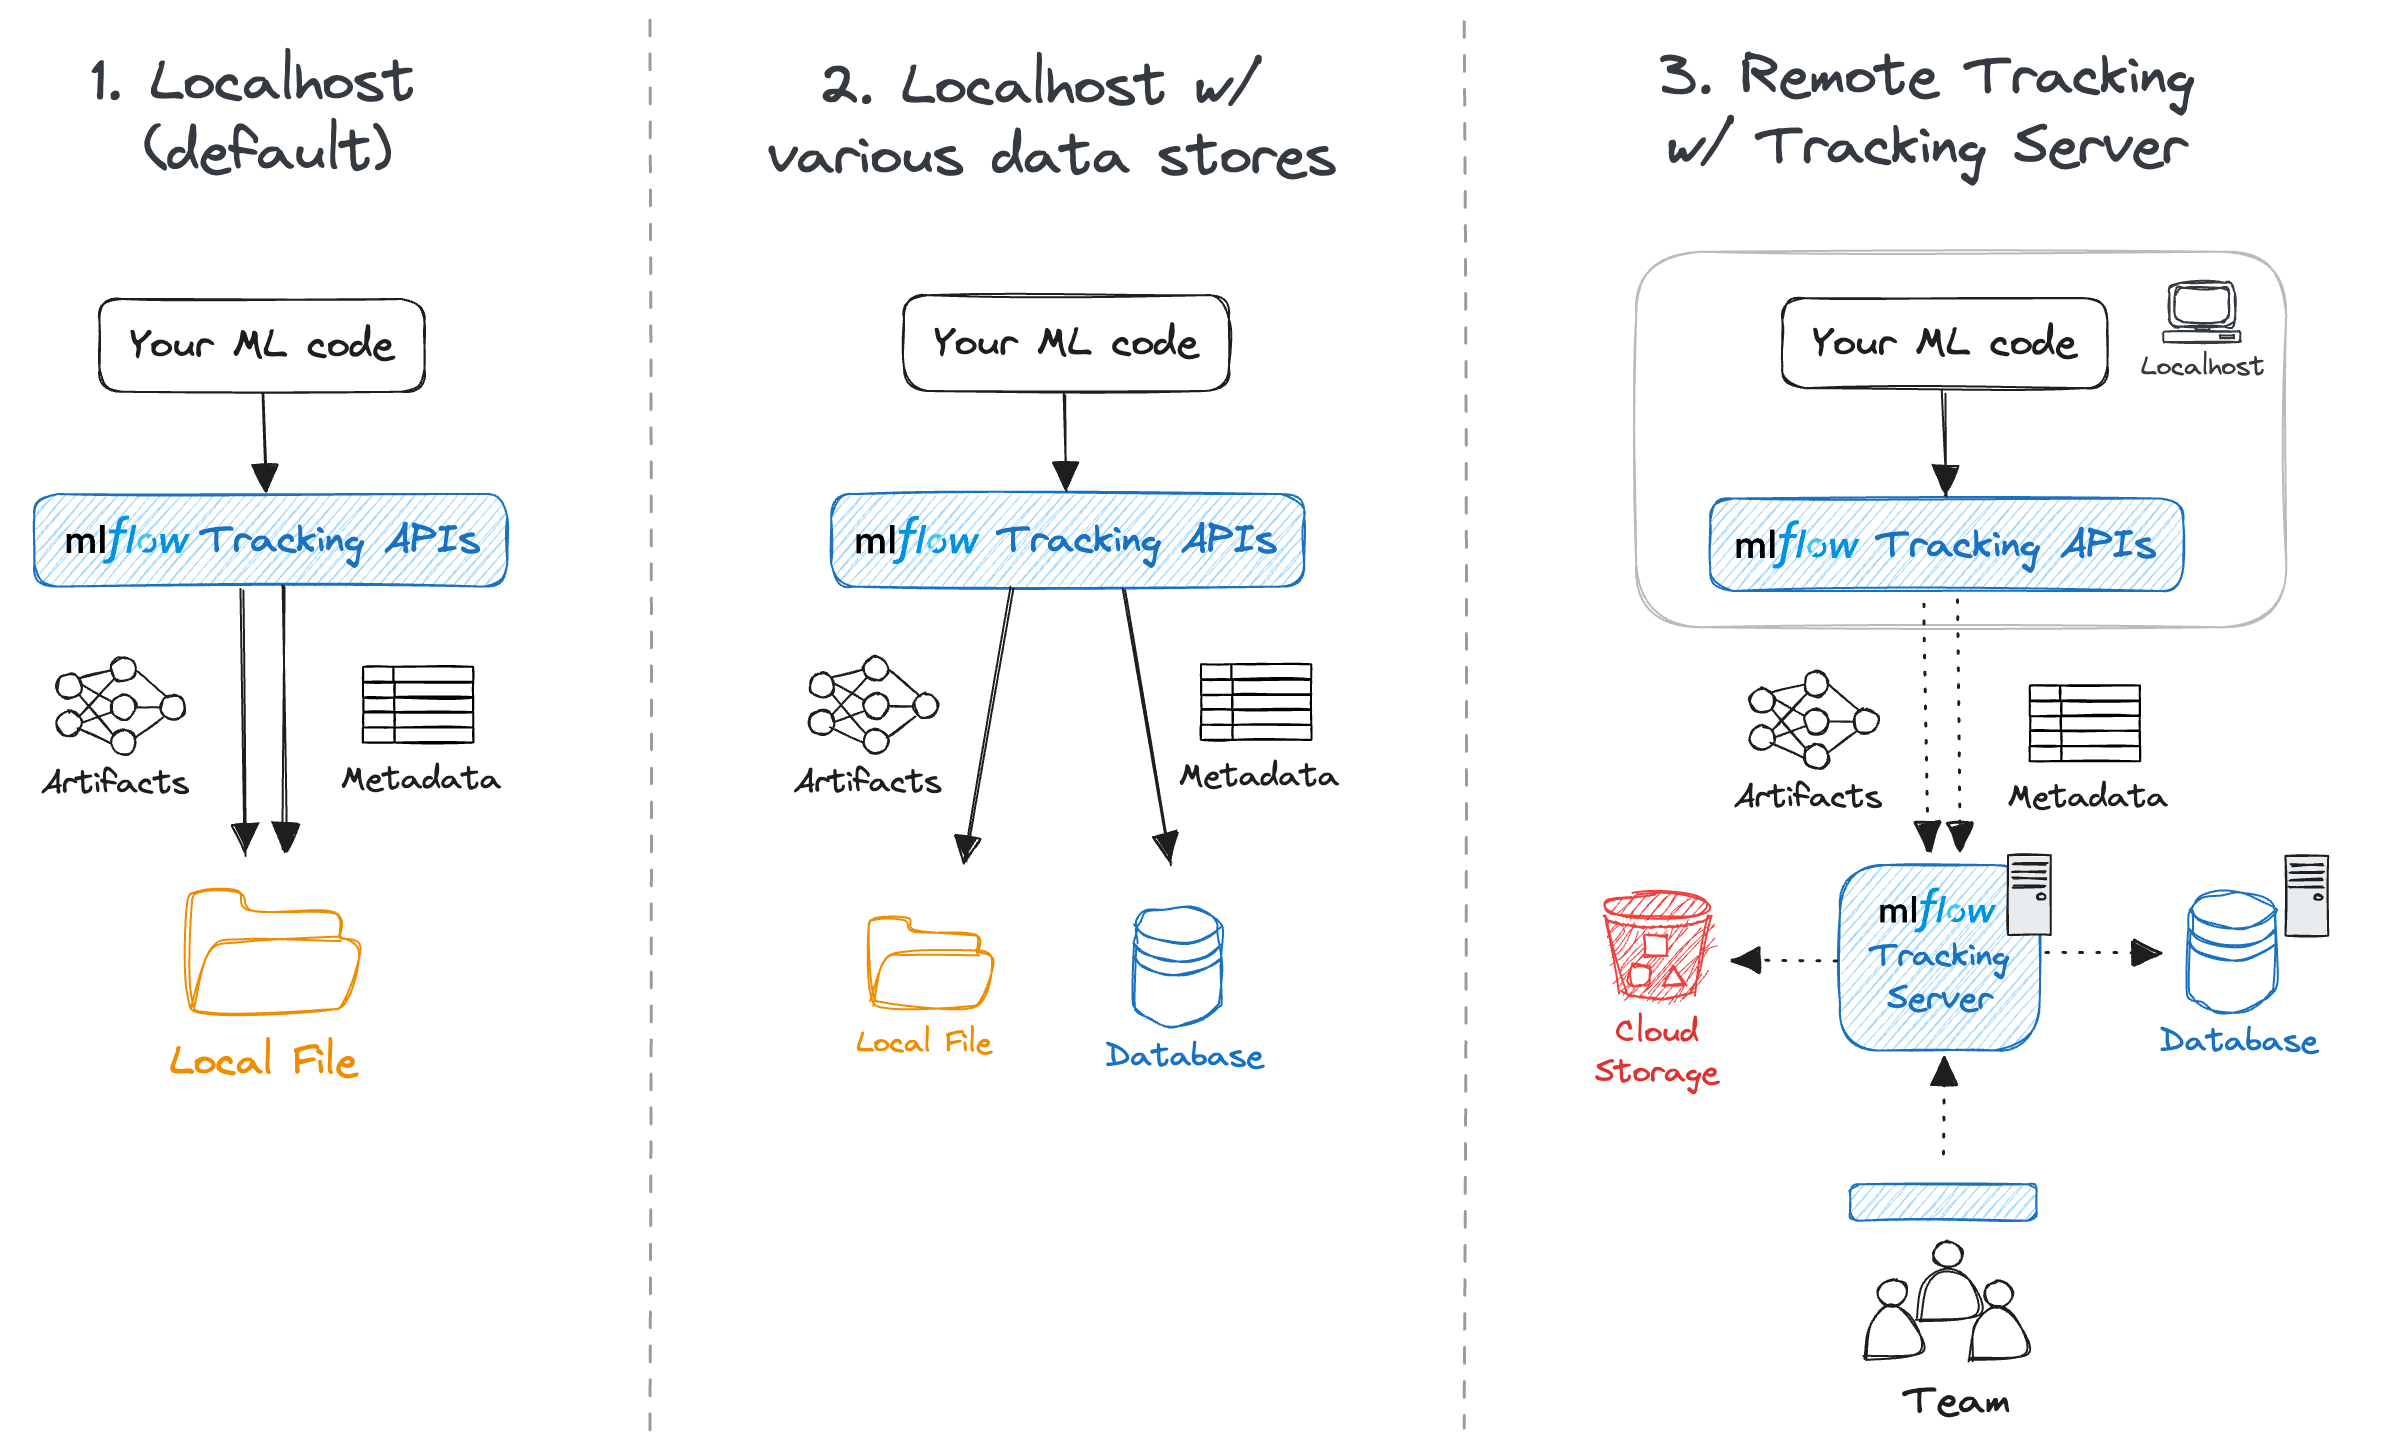
\includegraphics[width=0.86\textwidth,height=0.42\textheight,keepaspectratio]{images/mlops-foundations/mlflow_tracking_setup_overview.png}

    {\scriptsize Source: MLflow documentation, ``MLflow Tracking,''
    \href{https://mlflow.org/docs/latest/ml/tracking/}{mlflow.org/docs/latest/ml/tracking}.}

    \vspace{0.5em}
    \begin{itemize}
        \small
        \item \textbf{Metadata} (params, metrics, tags) goes to a database; \textbf{artifacts} (model files,
              plots) go to object storage. They are separate stores for a reason: one is small and queried,
              the other is large and streamed.
        \item Solo work: local files, zero setup. Team work: one shared tracking server, so ``my numbers''
              and ``your numbers'' live in the same place.
    \end{itemize}

\end{frame}

% --- SLIDE 6: THE UI ---
\begin{frame}{What You Get Back}

    \centering
    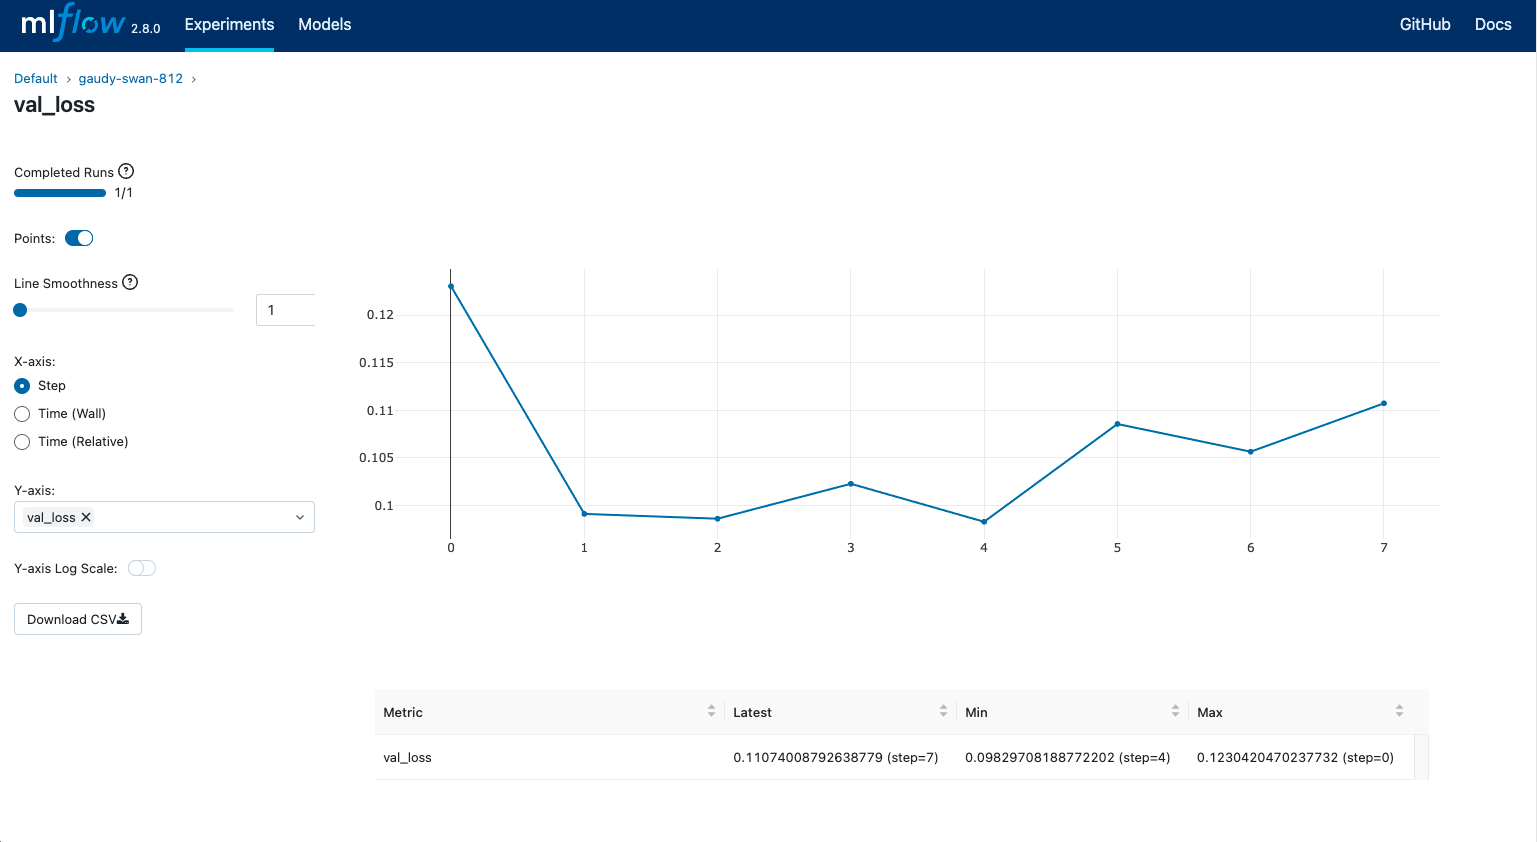
\includegraphics[width=0.78\textwidth,height=0.42\textheight,keepaspectratio]{images/mlops-foundations/mlflow_tracking_metrics_ui.png}

    {\scriptsize Source: MLflow documentation, ``MLflow Tracking'' --- metric view of a single run,
    \href{https://mlflow.org/docs/latest/ml/tracking/}{mlflow.org/docs/latest/ml/tracking}.}

    \vspace{0.5em}
    \begin{itemize}
        \small
        \item Sort and filter runs by any logged metric or parameter; overlay learning curves across runs.
        \item The payoff arrives about three weeks in, when someone asks ``why is production worse than
              your slide?'' and you can answer in thirty seconds.
    \end{itemize}

\end{frame}

% --- SLIDE 7: MLFLOW VS W&B ---
\begin{frame}{MLflow and Weights \& Biases, Side by Side}

    \centering
    \renewcommand{\arraystretch}{1.3}
    {\scriptsize
    \begin{tabular}{p{2.9cm}|p{4.2cm}|p{4.2cm}}
        \toprule
                        & \textbf{MLflow} & \textbf{Weights \& Biases} \\
        \midrule
        Model           & Open source (Apache~2.0), self-hosted or managed & Hosted SaaS; self-hosting on the
                          higher tiers \\
        Cost            & Free; you run the server & Free tier for personal use (corporate use excluded);
                          free Pro licences for academic research \\
        Setup           & \texttt{pip install mlflow} --- works offline & Account plus API key; logs to the cloud
                          by default \\
        Strength        & Registry, packaging, deployment story; lives inside your infrastructure &
                          Collaboration, reports, rich interactive dashboards, built-in sweeps \\
        HPO             & Bring your own (Optuna, Ray Tune) & \texttt{wandb sweeps} built in \\
        \bottomrule
    \end{tabular}}

    \vspace{0.24em}
    \begin{itemize}
        \scriptsize
        \item Both cover \textbf{runs, params, metrics, artifacts, registry}. The instrumentation in your
              training script is a handful of lines either way --- switching later is cheap.
        \item \textbf{Choose on constraints, not features:} can your data leave the building? Do you have
              someone to run a server? Is the audience your team or your customer?
        \item Others in the same shape: Neptune, Comet, ClearML, Aim, and the tracker built into most cloud
              ML platforms.
    \end{itemize}

    \vspace{0.09em}
    {\scriptsize Sources: \href{https://mlflow.org/docs/latest/}{MLflow documentation};
    \href{https://wandb.ai/site/pricing/}{W\&B pricing} (accessed 2026).}

\end{frame}

% --- SLIDE 8: HONEST COMPARISON ---
\begin{frame}{Comparing Runs Honestly}

    \begin{columns}[T]
        \begin{column}{0.5\textwidth}
            \begin{tcolorbox}[colback=red!5, colframe=red!50, title=\scriptsize Dishonest but common]
                \scriptsize
                \begin{itemize}
                    \item Report the best of 50 runs on the validation set as if it were an unbiased estimate.
                    \item Compare your tuned model against an untuned baseline.
                    \item Change three things at once and attribute the gain to your favourite one.
                    \item Report one seed.
                    \item Quietly drop the runs that did not work.
                \end{itemize}
            \end{tcolorbox}
        \end{column}
        \begin{column}{0.46\textwidth}
            \begin{tcolorbox}[colback=green!5, colframe=green!50!black, title=\scriptsize What to do instead]
                \scriptsize
                \begin{itemize}
                    \item Keep a \textbf{frozen test set} touched once, at the end.
                    \item Give the baseline the \emph{same} tuning budget.
                    \item Change one thing per run; the tracker makes this cheap.
                    \item Report mean $\pm$ spread over 3--5 seeds.
                    \item Keep failed runs, tagged. They are evidence.
                \end{itemize}
            \end{tcolorbox}
        \end{column}
    \end{columns}

    \vspace{0.21em}
    \begin{alertblock}{The baseline rule}
        Before any model goes to production, log a run for the \textbf{dumbest possible baseline}: predict
        the majority class, predict last week's value, use the existing business rule. Surprisingly often it
        wins --- and that is a result worth knowing before you build a serving stack.
    \end{alertblock}

\end{frame}
